\section{Appendix}
\begin{figure*}[h!]
    \centering
    \begin{subfigure}[b]{0.3\textwidth}
            
\includegraphics[width=\textwidth]{square_baseline}
            \caption{The baseline result}
            \label{fig:app_square_baseline}
    \end{subfigure}
    \begin{subfigure}[b]{0.3\textwidth}
            
\includegraphics[width=\textwidth]{square_out}
            \caption{The optimized result}
            \label{fig:app_square_out}
    \end{subfigure}
    \begin{subfigure}[b]{0.3\textwidth}
            
\includegraphics[width=\textwidth]{square}
            \caption{The original picture}
            \label{fig:app_square}
    \end{subfigure}

    \begin{subfigure}[b]{0.3\textwidth}
            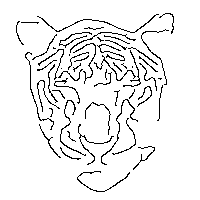
\includegraphics[width=\textwidth]{tiger_baseline}
            \caption{The baseline result}
            \label{fig:app_tiger_baseline}
    \end{subfigure}
    \begin{subfigure}[b]{0.3\textwidth}
            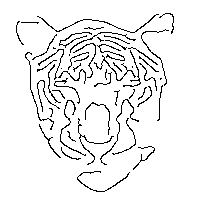
\includegraphics[width=\textwidth]{tiger_out}
            \caption{The optimized result}
            \label{fig:app_tiger_out}
    \end{subfigure}
    \begin{subfigure}[b]{0.3\textwidth}
            
\includegraphics[width=\textwidth]{tiger}
            \caption{The original picture}
            \label{fig:app_tiger}
    \end{subfigure}

    \begin{subfigure}[b]{0.3\textwidth}
            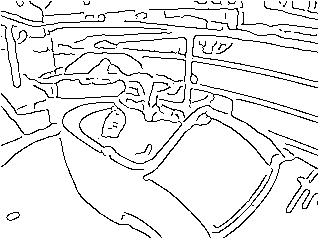
\includegraphics[width=\textwidth]{klomp_baseline}
            \caption{The baseline result}
            \label{fig:app_klomp_baseline}
    \end{subfigure}
    \begin{subfigure}[b]{0.3\textwidth}
            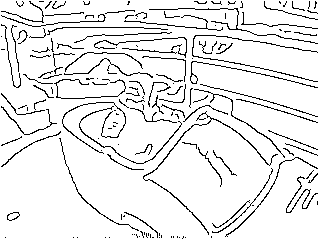
\includegraphics[width=\textwidth]{klomp_out}
            \caption{The optimized result}
            \label{fig:app_klomp_out}
    \end{subfigure}
    \begin{subfigure}[b]{0.3\textwidth}
            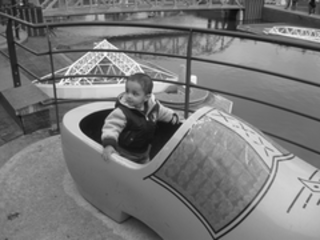
\includegraphics[width=\textwidth]{klomp}
            \caption{The original picture}
            \label{fig:app_klomp}
    \end{subfigure}
    \caption{The three different images used to test the implementation}
    \label{fig:imgdiff}
\end{figure*}
